% A CONSORT-style flowchart of a randomized controlled trial
% using the PGF/TikZ package
% Author  : Morten Vejs Willert (July 2010)
% License : Creative Commons attribution license
\documentclass{article}
\usepackage[latin1]{inputenc}
\usepackage[margin=0.25in]{geometry}
\usepackage{tikz}
\usetikzlibrary{positioning,shapes,arrows,fit}
\usepackage{caption}
\usepackage{amsmath}
\usepackage{verbatimbox}
\usepackage[framed]{matlab-prettifier}
\usepackage{filecontents}
\usepackage[scaled]{helvet}
\renewcommand\familydefault{\sfdefault} 
\usepackage[T1]{fontenc}
\usepackage[scaled]{beramono}
\usepackage{multicol}


% \tikzset{
%  font={\fontsize{10pt}{12}\selectfont}}

\begin{document}
\begin{center}
  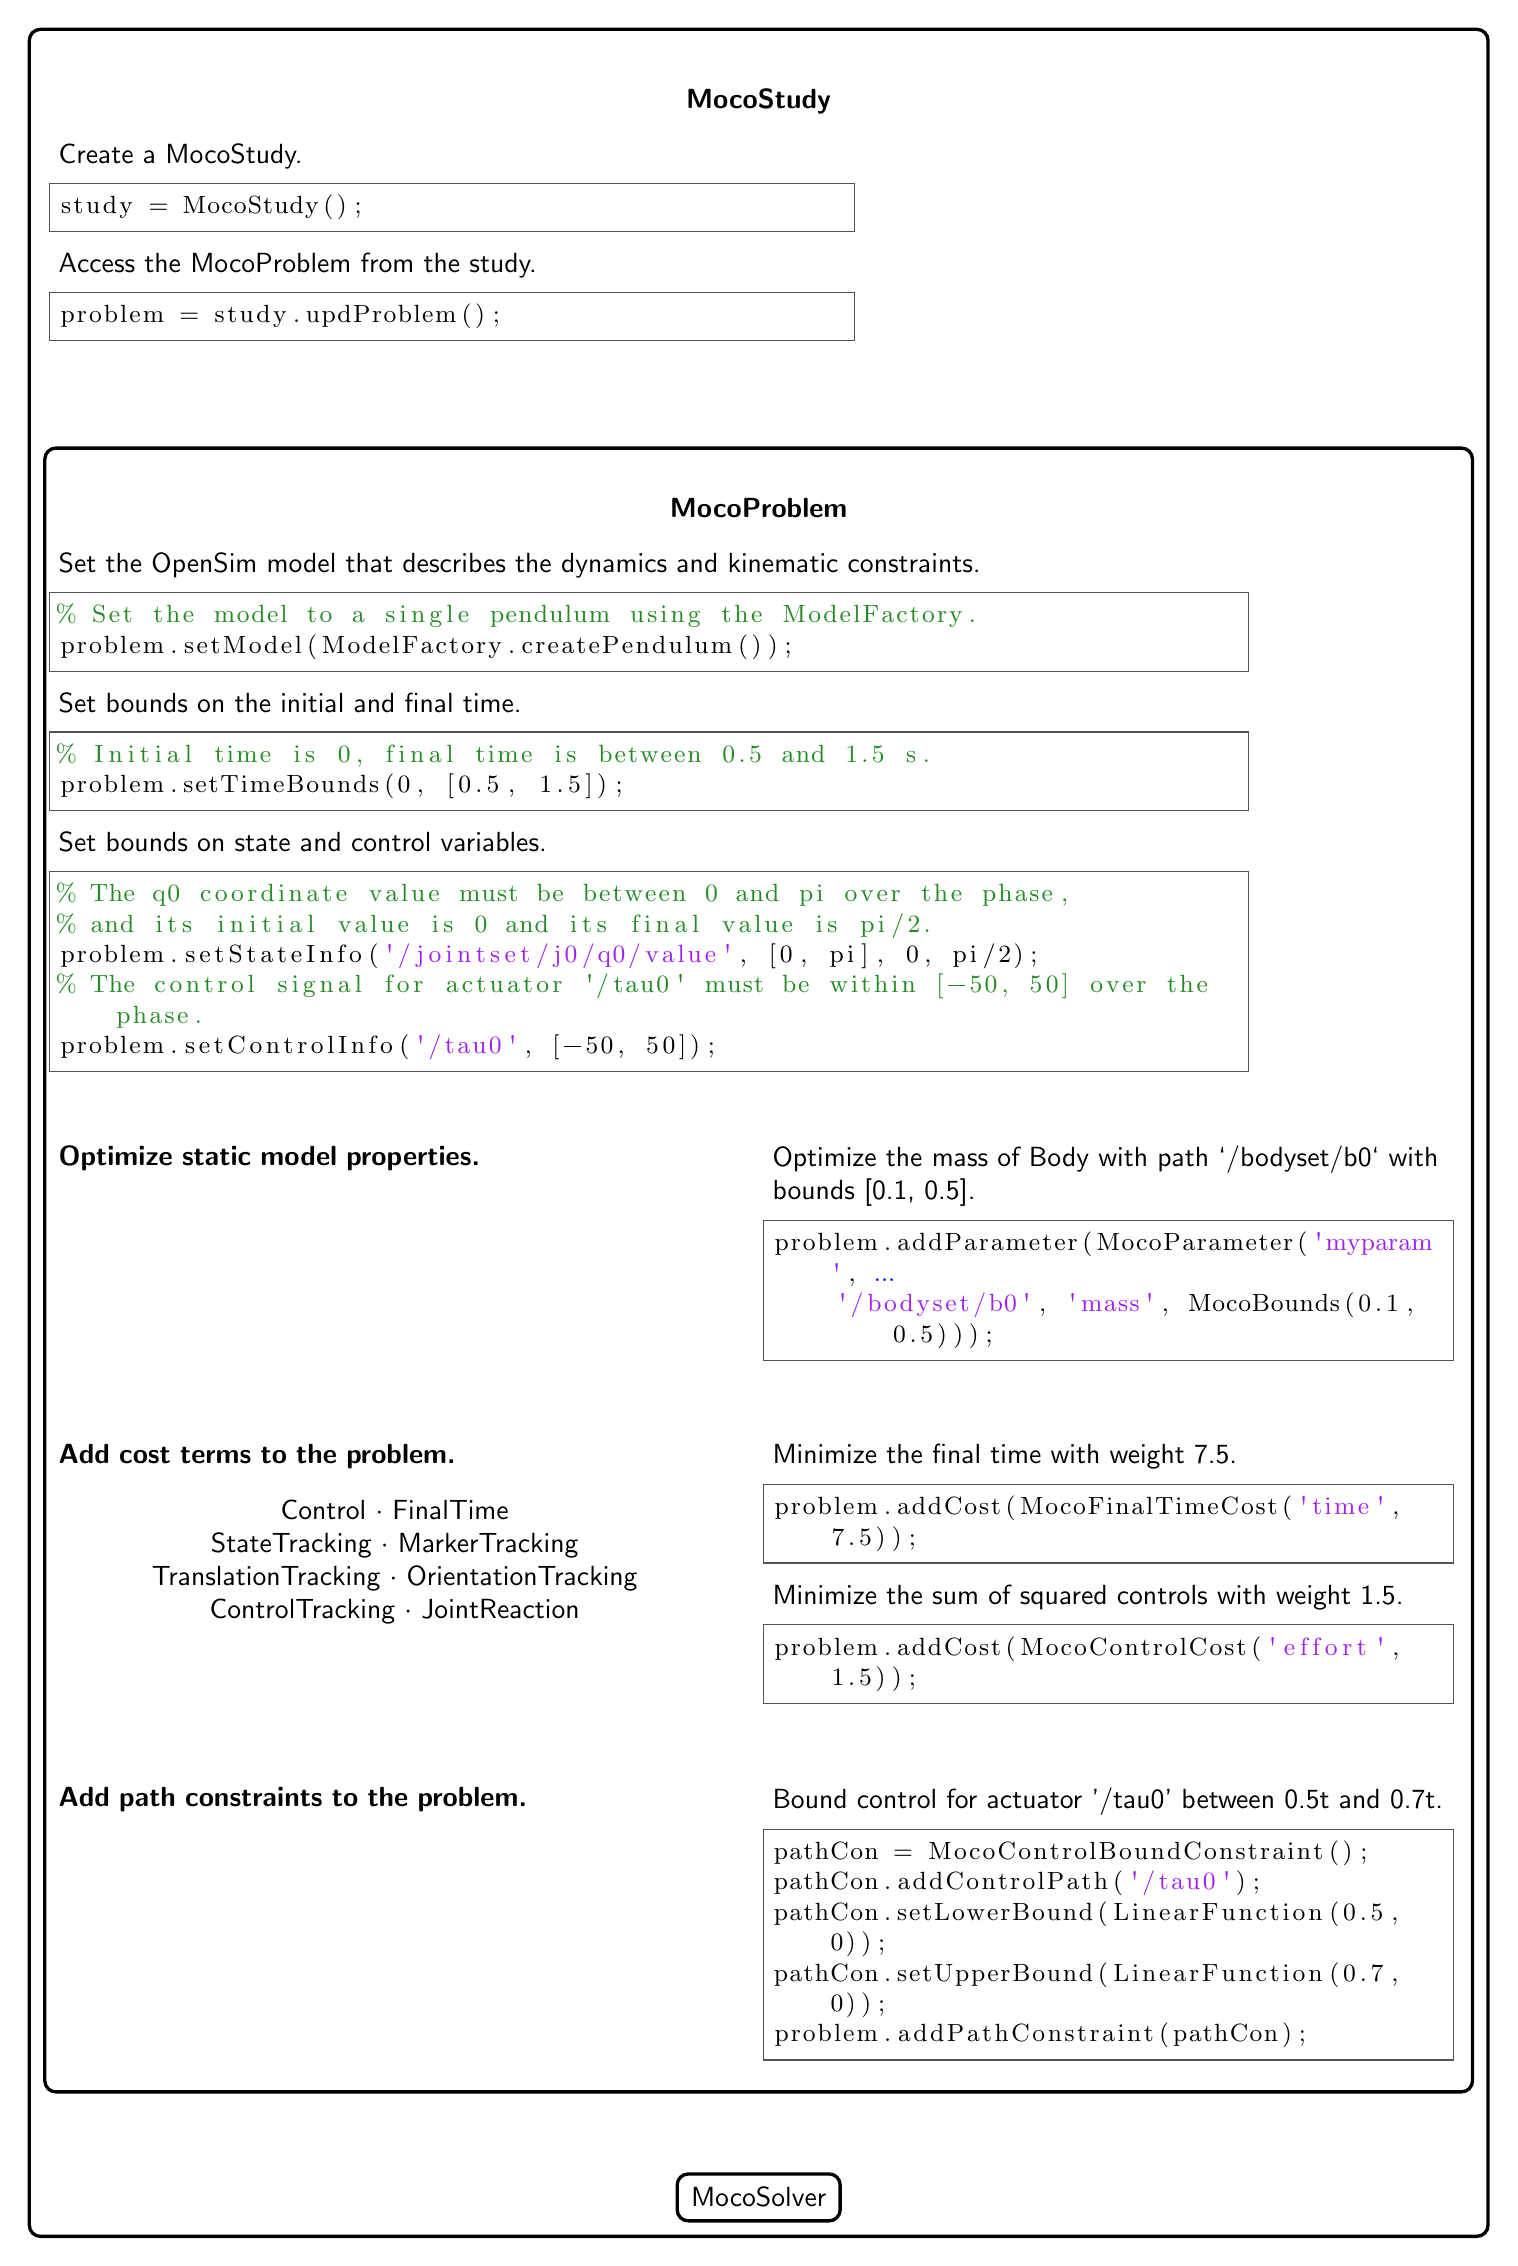
\begin{tikzpicture}[auto]
    
    
	\tikzstyle{object} = [draw=black, very thick,
    	rectangle, rounded corners, inner sep=5pt, inner ysep=5pt]
    
\node (studybody) [align=left, text width=7in] {
\begin{center}\textbf{MocoStudy}\end{center}
Create a MocoStudy.
\begin{lstlisting}[style=Matlab-editor, basicstyle=\mlttfamily\small, linewidth=10cm]
study = MocoStudy();
\end{lstlisting}
Access the MocoProblem from the study.
\begin{lstlisting}[style=Matlab-editor, basicstyle=\mlttfamily\small, linewidth=10cm]
problem = study.updProblem();
\end{lstlisting}
};
    
    \node (problem) [object, below=of studybody, align=left, text width=7in] {
    \begin{center}\textbf{MocoProblem}\end{center}
Set the OpenSim model that describes the dynamics and kinematic constraints.
\begin{lstlisting}[style=Matlab-editor, basicstyle=\mlttfamily\small, linewidth=15cm]
% Set the model to a single pendulum using the ModelFactory.
problem.setModel(ModelFactory.createPendulum());
\end{lstlisting}
Set bounds on the initial and final time.
\begin{lstlisting}[style=Matlab-editor, basicstyle=\mlttfamily\small, linewidth=15cm]
% Initial time is 0, final time is between 0.5 and 1.5 s.
problem.setTimeBounds(0, [0.5, 1.5]);
\end{lstlisting}
Set bounds on state and control variables.
\begin{lstlisting}[style=Matlab-editor, basicstyle=\mlttfamily\small, linewidth=15cm]
% The q0 coordinate value must be between 0 and pi over the phase, 
% and its initial value is 0 and its final value is pi/2.
problem.setStateInfo('/jointset/j0/q0/value', [0, pi], 0, pi/2);
% The control signal for actuator '/tau0' must be within [-50, 50] over the phase.
problem.setControlInfo('/tau0', [-50, 50]);
\end{lstlisting}
\begin{multicols}{2}% 2-column layout
  \begin{minipage}{0.48\textwidth}
\textbf{Optimize static model properties.}
  \end{minipage}
  \vfill\null
\columnbreak
Optimize the mass of Body with path `/bodyset/b0` with bounds [0.1, 0.5].
\begin{lstlisting}[style=Matlab-editor, basicstyle=\mlttfamily\small, linewidth=0.48\textwidth]
problem.addParameter(MocoParameter('myparam', ...
    '/bodyset/b0', 'mass', MocoBounds(0.1, 0.5)));
\end{lstlisting}
\end{multicols}
\begin{multicols}{2}% 2-column layout
  \begin{minipage}{0.48\textwidth}
\textbf{Add cost terms to the problem.}
\begin{center}
Control $\cdot $ FinalTime\\
StateTracking $\cdot$ MarkerTracking\\
TranslationTracking $\cdot$ OrientationTracking\\
ControlTracking $\cdot$ JointReaction
\end{center}
  \end{minipage}
  \vfill\null
\columnbreak
Minimize the final time with weight 7.5.
\begin{lstlisting}[style=Matlab-editor, basicstyle=\mlttfamily\small, linewidth=0.48\textwidth]
problem.addCost(MocoFinalTimeCost('time', 7.5));
\end{lstlisting}
Minimize the sum of squared controls with weight 1.5.
\begin{lstlisting}[style=Matlab-editor, basicstyle=\mlttfamily\small, linewidth=0.48\textwidth]
problem.addCost(MocoControlCost('effort', 1.5));    
\end{lstlisting}
\end{multicols}
\begin{multicols}{2}% 2-column layout
  \begin{minipage}{0.48\textwidth}
\textbf{Add path constraints to the problem.}
  \end{minipage}
  \vfill\null
\columnbreak
Bound control for actuator '/tau0' between 0.5t and 0.7t.
\begin{lstlisting}[style=Matlab-editor, basicstyle=\mlttfamily\small, linewidth=0.48\textwidth]
pathCon = MocoControlBoundConstraint();
pathCon.addControlPath('/tau0');
pathCon.setLowerBound(LinearFunction(0.5, 0));
pathCon.setUpperBound(LinearFunction(0.7, 0));
problem.addPathConstraint(pathCon);
\end{lstlisting}
\end{multicols}
};
    
    \node (solver) [object, below=of problem] {MocoSolver};
    
    
    \node (study) [object, fit={(studybody) (problem) (solver)}] {};
%      	\begin{equation*}
%      	    \begin{alignat*}{2}
%        \mbox{minimize}
%         \quad & \sum_j w_{E,j} \left(J_{E,j}(t_0, t_f, y_0, y_f, x_{0}, x_{f}, \lambda_0, \lambda_f, p)
%         + \int_{t_0}^{t_f} J_{I,j}(t, y, x, \lambda, p)~dt\right) &&  \\
%        \mbox{subject to}
%         \quad & \dot{q} = u \\
%         & M(q, p)\dot{u} + G(q, p)^T \lambda = f_{\textrm{app}}(t, y, x, p) - f_{\textrm{bias}}(q, u, p) \\
%         & \dot{z}(t) = f_{\textrm{aux}}(t, y, x, \lambda, p) \\
%         & 0 = \phi(q, p) \\
%         & 0 = \nu(q, u, p) \\
%         & 0 = \alpha(q, u, \dot{u}, p) \\
%         & g_{L} \leq g(t, y, x, \lambda, p) \leq g_{U} \\
%         & y_{0,L} \leq y_0 \leq y_{0,U} \\
%         & x_{0,L} \leq x_0 \leq x_{0,U} \\
%         & y_{f,L} \leq y_f \leq y_{f,U} \\
%         & x_{f,L} \leq x_f \leq x_{f,U} \\
%         \mbox{with respect to} \quad
%         & y \in [y_{L}, y_{U}] \\
%         & x \in [x_{L}, x_{U}] \\
%         & p \in [p_{L}, p_{U}] \\
%         & t_0 \in [t_{0,L}, t_{0,U}] \\
%         & t_f \in [t_{f,L}, t_{f,U}]
%    \end{alignat*}
%    \end{equation*}
  \end{tikzpicture}
\end{center}
\end{document}



%    block_center/.style ={
%    	rectangle, rounded corners,
%    	draw=black, very thick,
%      	text width=8em, text centered,
%      	minimum height=4em,
%      	inner sep=10pt,
%      	inner ysep=10pt,
%      	% minimum width=50em,
%      },
%    block_left/.style ={
%    	rectangle, rounded corners,
%    	draw=black, very thick,
%      	text width=8em,
%      	minimum height=4em,
%      	inner sep=10pt,
%      	inner ysep=10pt,
%      	minimum width=50em
%      	},
%    block_noborder/.style ={rectangle, draw=none, thick, fill=none,
%      text width=18em, text centered, minimum height=1em},
%    block_assign/.style ={rectangle, draw=black, thick, fill=white,
%      text width=18em, text ragged, minimum height=3em, inner sep=6pt},
%    block_lost/.style ={rectangle, draw=black, thick, fill=white,
%      text width=16em, text ragged, minimum height=3em, inner sep=6pt},
%      line/.style ={draw, thick, -latex', shorten >=0pt}]
%
%
